\documentclass[11pt]{article}
\usepackage[margin=2.0cm]{geometry}
\usepackage{graphicx}
\graphicspath{{figures/}{../figures/}}
\usepackage{amsmath,amssymb,amsfonts}
\usepackage{multirow}
\usepackage{booktabs}
\usepackage{xr-hyper}
\usepackage{hyperref}
\externaldocument[M-]{manuscript}
\usepackage[linesnumbered,ruled,vlined]{algorithm2e}
\usepackage[authoryear,round]{natbib}
% Notation macros: one definition per compound symbol.
\newcommand{\Rsys}{R_{\mathrm{sys}}}\newcommand{\Rtarget}{R_{\mathrm{target}}}
\newcommand{\kag}{k^{\alpha}(\gamma)}\newcommand{\WS}{\tilde{W}_S}\newcommand{\Zsuf}{Z^{\mathrm{suf}}}
\newcommand{\new}[1]{#1}
\renewcommand{\thesection}{S\arabic{section}}
\renewcommand{\theequation}{S.\arabic{equation}}
\renewcommand{\thetable}{S\arabic{table}}
\renewcommand{\thefigure}{S\arabic{figure}}
\title{Supplementary Material\\[4pt]
\large Reliability Optimization of Weighted $k$-out-of-$n$:G Systems under Dual Fuzziness}
\author{\ifdefined\anonbuild\else Kadir Sar\i kaya\fi}
\date{}
\begin{document}
\maketitle
\sloppy

\noindent This document collects material that supports the main article without being needed to
follow its primary argument: a mechanical trace of the dual-fuzzy evaluation rule, the static
reliability and both phases of the exact search (Section~\ref{sec:supp_trace}); the script-level provenance of every
reported result, the verification checks and the computational environment (Section~\ref{sec:supp_pipeline}); the
verification record of the uncertainty-theory oracle (Section~\ref{sec:supp_oracle}); the Pharmaceutical-derived instance
with the uncertainty-theory comparison (Section~\ref{sec:supp_pharma}); the Fyffe-derived instance (Section~\ref{sec:supp_fyffe}); further
results on the IEEE RTS-79 case study (Section~\ref{sec:supp_rts}); and the details of the model baselines
(Section~\ref{sec:supp_baselines}). Section numbers here are prefixed S and are cited from the main text as S1--S7.

\section{Illustrative Example: Exact Calculation Trace} \label{sec:supp_trace}

This section traces the evaluation rule and the static reliability on a three-component system. Consider three components with reliabilities $p_1 = 0.95$, $p_2 = 0.90$ and $p_3 = 0.85$. Their functional capacities (weights) are modeled directly as Triangular Fuzzy Numbers (TFNs), defined via their lower, modal, and upper bounds $\tilde{w}_i = (w_{i,L}^0, w_i, w_{i,U}^0)$:
\begin{itemize}
    \item $\tilde{w}_1 = (4.32, 4.80, 5.28)$
    \item $\tilde{w}_2 = (4.50, 5.00, 5.50)$
    \item $\tilde{w}_3 = (4.50, 5.00, 5.50)$
\end{itemize}

Simultaneously, the system's operational target is defined by an expert-elicited fuzzy baseline threshold:
\begin{equation}
    \tilde{k} = (6.0, 8.0, 10.0)
\end{equation}


To evaluate the success condition ($\WS \tilde{\ge} \tilde{k}$), we apply the Hurwicz evaluation rule. Under the pessimistic evaluation stance ($\gamma = 0$), which by Proposition~\ref*{M-prop:chance} corresponds to the necessity ranking criterion of \citet{DuboisPrade1983} and \citet{InuiguchiRamik2000}, a subset is accepted only if its lower capacity endpoint is at least the upper endpoint of the threshold, $W_{S,L}^\alpha \ge k_U^\alpha$.

Assume a configuration that engages all three modules ($\mathbf{x} = [1,1,1]$). We trace its static reliability at the cut level $\alpha = 0.5$.

\textbf{1. Evaluating Component Capacities and Subset Weight}

First, we extract the $\alpha=0.5$ lower-bound capacities for the active components using the algebraic interval transformation $w_{i,L}^\alpha = w_{i,L}^0 + \alpha(w_i - w_{i,L}^0)$:
\begin{itemize}
    \item $w_{1,L}^{0.5} = 4.32 + 0.5(4.80 - 4.32) = 4.56$
    \item $w_{2,L}^{0.5} = 4.50 + 0.5(5.00 - 4.50) = 4.75$
    \item $w_{3,L}^{0.5} = 4.50 + 0.5(5.00 - 4.50) = 4.75$
\end{itemize}
When all three components are operational (forming subset $S = \{1,2,3\}$), the aggregated pessimistic boundary evaluates to $W_{S,L}^{0.5} = 4.56 + 4.75 + 4.75 = 14.06$.

\textbf{2. Extracting Threshold and Checking Subset Feasibility}

Next, we extract the upper endpoint of the threshold:
\begin{equation}
    k_U^{0.5} = 10.0 - 0.5(10.0 - 8.0) = 9.0
\end{equation}


Evaluating the core success condition ($W_{S,L}^\alpha \ge k_U^\alpha$) yields:
\begin{equation}
    14.06 \ge 9.0 \quad \text{\textbf{(Condition Satisfied)}}
\end{equation}
The full set $S=\{1,2,3\}$ is therefore accepted at $\alpha=0.5$. 

\textbf{3. Determining Functional Subsets}

We evaluate if the system survives the failure of individual modules. If component 1 fails, the remaining aggregated capacity is $W_{S',L}^{0.5} = 4.75 + 4.75 = 9.5$. Since $9.5 \ge 9.0$, the system remains operational. Similarly, the removal of component 2 or component 3 yields remaining weights of $9.31 \ge 9.0$. Thus, all subsets with at least two components ($S \in \{\{1,2,3\}, \{1,2\}, \{1,3\}, \{2,3\}\}$) are validated success states.

\textbf{4. Calculating the Static Reliability}

The static reliability $\Rsys^{0.5,0}$ of Equation~(\ref*{M-eq:static}) of the main article sums the probabilities of
the four mutually exclusive success configurations found in Step~3:
\begin{align}
    \Rsys^{0.5,0} &= p_1p_2p_3 + p_1p_2(1-p_3) + p_1p_3(1-p_2) + p_2p_3(1-p_1) \nonumber \\
    &= 0.72675 + 0.12825 + 0.08075 + 0.03825 = 0.974 .
\end{align}

\textbf{Conclusion of the Trace}

The $\alpha$-cut endpoints of the capacities and of the threshold determine which subsets are accepted,
and the static reliability ($0.974$) follows from the probabilities of the accepted subsets.

\subsection{Optimization Trace: The Two-Phase Exact Search}

We trace Algorithm~\ref*{M-alg:exact_solver} of the main article on the three components above, now read as three subsystems with catalogs, in the cell $(\alpha,\gamma)=(0.5,0)$, which by Proposition~\ref*{M-prop:chance} is the necessity constraint $N(\WS\ge\tilde{k})\ge 0.5$. Subsystem~1 offers two options: option~1, the unit above ($c_{1,1}=10$, $p_{1,1}=0.95$, $\tilde{w}_{1,1}=(4.32, 4.80, 5.28)$), and option~2, a larger and more reliable unit ($c_{1,2}=20$, $p_{1,2}=0.97$, $\tilde{w}_{1,2}=(4.95, 5.50, 6.05)$). Subsystems~2 and~3 each offer one option, the units above at cost $15$. The target is $\Rtarget=0.90$. Design $[1,1,1]$ costs $40$ and design $[2,1,1]$ costs $50$. The trace is generated by \texttt{supp\_trace\_v11.py} (Section~\ref{sec:supp_pipeline}).

\textbf{Phase 0: effective values and suffix tables.} At $(0.5,0)$ the threshold is $k^{0.5}(0)=k_U^{0.5}=9.0$ and every effective capacity is a lower endpoint: $w_{1,1}=4.56$, $w_{1,2}=5.225$, $w_{2,1}=w_{3,1}=4.75$. The largest capacity that subsystems~2 and~3 can add is $W^{\mathrm{max}}_1=9.5$. Because these subsystems have one option each, $\Zsuf_1(q)=30$ for every $q\le 9.5$.

\textbf{Incumbent seed.} The greedy design starts from the largest unit of every subsystem, $[2,1,1]$, whose accepted subsets are those with at least two units, so that $\Rsys^{0.5,0}([2,1,1])=0.9784$. Replacing option~2 by the cheaper option~1 keeps the target met, $\Rsys^{0.5,0}([1,1,1])=0.974$ (Step~4 above), and no further substitution lowers the cost. Phase~1 therefore starts with the incumbent $Z^*=40$.

\textbf{Phase 1: cost certification.} Options are explored in ascending cost order, so the search first branches on option~1 of subsystem~1: $Z_{\mathrm{next}}=10$ and $q_{\mathrm{next}}=9.0-4.56=4.44$. The cost bound gives $Z_{\mathrm{next}}+\Zsuf_1(4.44)=40$, which equals the incumbent and therefore does not prune: by Theorem~\ref*{M-thm:bb_bounds}(ii) only a strictly larger bound prunes, since an equal-cost completion may still win at the secondary level. The capacity bound $4.56+9.5=14.06\ge 9.0$ and the optimistic reliability bound of Theorem~\ref*{M-thm:rel_bound}, here $0.974\ge 0.90$, do not prune either. The two single-option subsystems follow, and the leaf $[1,1,1]$ meets the target, so $Z^*=\min(40,40)=40$. The search then returns to option~2 of subsystem~1: $Z_{\mathrm{next}}=20$, $q_{\mathrm{next}}=9.0-5.225=3.775$, and $20+\Zsuf_1(3.775)=50>40$. Theorem~\ref*{M-thm:bb_bounds}(ii) prunes the subtree before its distribution is convolved, although its only design, $[2,1,1]$, is the more reliable one. Phase~1 ends with the certified minimum cost $Z^*=40$.

\textbf{Phase 2: iso-cost reliability maximization.} With $Z^*=40$ fixed, the traversal is repeated with the same tests. The only leaf of cost $40$ is $[1,1,1]$, so $\mathbf{x}^*=[1,1,1]$ and $R^*=0.974$, and option~2 of subsystem~1 is pruned again by the cost bound.

\textbf{Result.} The algorithm returns $(\mathbf{x}^*,Z^*,R^*)=([1,1,1],\,40,\,0.974)$, the lexicographic optimum of Theorem~\ref*{M-thm:optimality}: the cheapest design that meets the target, not the most reliable one. Without the seed, Phase~1 would start from $Z^*=\infty$, reach the same leaf first and prune option~2 in the same way.

\section{Computational Pipeline, Verification Checks and Environment} \label{sec:supp_pipeline}

\subsection{Script-level provenance}

\begin{enumerate}
\item \texttt{run\_campaign\_v2.py}: the $30$-cell grid on each of the two derived instances ($60$ cells) solved with the interpreted backend; it is kept as a cross-check of the compiled backend, and the reported results of these instances come from \texttt{generate\_benchmark\_tables\_v6.py}. Writes \texttt{campaign\_v2\_default.json}.
\item \texttt{run\_measure\_family.py}: closed forms for possibility, necessity and credibility, the chance-constraint equivalence sweep of Proposition~\ref*{M-prop:chance}, and the decomposition identity of Equation~(\ref*{M-eq:decomposition}) of the main article.
\item \texttt{parametric\_stability.py}: the complete parametric solution over $[0,1]^2$, including the recovery check against the archived audit cells.
\item \texttt{run\_scaling\_campaign.py}: the unreduced interpreted scaling campaign (Regime~1 of Table~\ref*{M-tab:ablation} of the main article) for $n \in \{8, 10, 12, 16, 20, 24, 28, 32\}$ with a $12$~s budget per instance; it certifies every instance up to $n=12$, and all larger instances time out. The cells $n=14$ and $n=18$ of that regime were measured separately under the same budget and are recorded, with a note, in \texttt{ablation\_v6.json}.
\item \texttt{run\_scaling\_campaign\_v4.py}: the synthetic scaling family under C++ and Theorem~\ref*{M-thm:reduction} reduction, with the reduced-versus-unreduced agreement verification.
\item \texttt{ablation\_v5.py}: isolates the algorithmic dimensional reduction from compilation and budget increases at $n=14$, computing iso-budget scaling frontiers.
\item \texttt{run\_baseline\_matched\_v6.py}: the budget-matched genetic-algorithm comparison under both protocols.
\item \new{\texttt{run\_uncertainty\_baseline\_v6.py}: the oracle-substitution experiment against Liu's uncertainty theory, including the reproduction of the published worked example and the numerical admissibility check of the substituted bound.}
\item \texttt{verify\_pharma\_oracle.py}: independent oracle verification on the 10-subsystem pharmaceutical plant benchmark.
\item \texttt{verify\_fyffe\_dp.py}: independent dynamic programming verification of the adapted Fyffe benchmark solutions.
\item \texttt{verify\_fyffe\_original.py}: reproduces the original published Fyffe et al. (1968) Table~III optimum under their exact series-parallel model.
\item \texttt{verify\_fyffe\_provenance\_v6.py}: the three provenance claims for the Fyffe benchmark: entry-by-entry agreement of the archived Table~I with the published scan, reproduction of the Table~III optimum under the source's own series-redundancy model, and the verbatim/synthetic breakdown of the adapted catalog. Writes \texttt{results/generated/fyffe\_provenance\_v6.json}.
\item \texttt{generate\_benchmark\_tables\_v6.py}: the two benchmark result tables, rebuilt from the current solver with the necessity and possibility reliabilities of each prescribed design.
\item \texttt{run\_audits\_v6.py}: the verification checks (ii)--(ix) below: the closed-form grid comparison, the chance-constraint correspondence sweep, the exact-rational factorization check, the credibility audit under symmetric and asymmetric spreads, and the leaf/node accounting. Writes a single artifact, \texttt{results/generated/audits\_v6.json}, recording the sampling domain, seed and outcome of each check.
\item \new{\texttt{generate\_figures\_v6.py}: Figure~\ref*{M-fig:insight_policy} of the main article and the figures of Sections~\ref{sec:supp_fyffe} and~\ref{sec:supp_rts}, drawn from the artifacts, \texttt{benchmark\_power\_rts.json} and \texttt{benchmark\_tables\_v6.json}.}
\item \new{\texttt{plot\_parametric\_partition\_v7.py}: the complete parametric solution of the IEEE RTS-79 fleet over the policy square; it checks that the closed-form boundaries of Corollary~\ref*{M-cor:partition} lie on the level sets $\kappa = T$ and that every cell of the $30$-cell grid falls in a region whose design and cost match the certified optimum of that cell.}
\item \new{\texttt{run\_power\_rts\_campaign\_v7.py}: the $30$-cell exact optimization campaign on the IEEE RTS-79 power generation fleet case study. Writes \texttt{results/generated/benchmark\_power\_rts.json} and \texttt{results/generated/table\_power\_rts.tex}.}
\item \texttt{run\_power\_rts\_unit\_specific\_v7.py}: the unit-specific capacity-spread experiment on the IEEE RTS-79 fleet: all $30$ policy cells solved by the unreduced exact search (time limit $600$\,s per cell), the $2\times2$ decomposition of each changed cell into thermal and hydro effects, and the hydro and thermal spread sweeps. Writes \texttt{results/generated/rts\_unit\_specific\_v7.json} and the corresponding table. The $30$ unit-specific solves take $1{,}363$~s of solver time in total, the slowest $234$~s; the decomposition and sweep runs are not timed.
\item \new{\texttt{verify\_unit\_specific\_bruteforce\_v8.py}: an independent check of the unit-specific experiment: exhaustive enumeration of all $3^{10}$ fleets in exact rational arithmetic, sharing no code with the compiled search, for the common-spread optimum at $(0.3,0.7)$, the unit-specific optima at $(0,0)$, $(0.3,0)$ and $(0.3,0.7)$, and the \$171\,M fleet selected under perturbed spreads, which it also confirms to be the crisp optimum of no integer threshold. Writes \texttt{results/generated/unit\_specific\_bruteforce\_v8.json}.}
\item \new{\texttt{crisp\_vs\_fuzzy\_v8.py}: the crisp and dual-fuzzy reliability of the seven RTS-79 designs of the parametric solution, with capacities only, demand only and both sides fuzzified, in the necessity cell and the optimistic boundary cell $(0,1)$ (exact rational enumeration). Writes \texttt{results/generated/crisp\_vs\_fuzzy\_v8.json} and \texttt{manuscript/table\_crisp\_vs\_fuzzy.tex}.}
\item \new{\texttt{policy\_menu\_v8.py}: the design menu of the IEEE RTS-79 parametric solution (cost, necessity and possibility reliabilities and area share of each of the seven designs), the budget inversion and the $\gamma$ intervals of Corollary~\ref*{M-cor:partition} reported in Sections~\ref*{M-sec:parametric} and~\ref*{M-sec:managerial} of the main article. Writes \texttt{results/generated/policy\_menu\_v8.json} and \texttt{manuscript/table\_policy\_menu.tex}.}
\item \new{\texttt{run\_delta\_sensitivity\_v7.py}: continuous sensitivity analysis over capacity spread $\delta \in [0.02, 0.20]$ and asymmetric seasonal thermal derating regimes on the IEEE RTS-79 fleet. Writes \texttt{results/generated/delta\_sensitivity\_v7.json} and generates \texttt{figures/fig\_delta\_sensitivity.pdf}.}
\item \new{\texttt{rts\_true\_frontier\_v9.py} and \texttt{plot\_true\_frontier\_v9.py}: exhaustive enumeration of all $3^{10} = 59{,}049$ candidate RTS-79 fleet designs (double precision) to construct the cost--necessity frontier (total cost $Z$ against $R_N$) with and without the crisp adequacy constraint $R_{\mathrm{modal}} \ge 0.95$, the crisp adequacy of the menu designs, the adequacy-constrained frontier table of Section~\ref*{M-sec:frontier} of the main article (\texttt{manuscript/table\_adequate\_frontier.tex}) and Figure~\ref*{M-fig:true_pareto_frontier}. Writes \texttt{results/generated/rts\_true\_frontier\_v9.json} and generates \texttt{figures/fig\_true\_pareto\_frontier.pdf}.}
\item \texttt{replication\_table\_v10.py}: the replication table of Section~\ref*{M-sec:parametric} of the main article (case study and the two literature-derived instances), read from the archived grid and parametric artifacts; it checks that every grid optimum belongs to the parametric library. On the region of the policy square whose optimum is at no grid cell it reports the share on which the design of the nearest grid cell does not meet the reliability target, the largest cost excess of the cheapest grid design that does, and the area on which no grid design meets it. Each region $\{\lceil\kappa(\alpha,\gamma)\rceil = T\}$ is, at fixed $\alpha<1$, the interval of $\gamma$ between the boundaries of Corollary~\ref*{M-cor:partition} for $T$ and $T-1$, so its area is a one-dimensional integral in $\alpha$ (midpoint rule, $2\times10^5$ nodes); whether a design meets the target at $T$ is checked with its crisp reliability. Writes \texttt{results/generated/replication\_v10.json} and \texttt{manuscript/table\_replication.tex}.
\item \new{\texttt{rts\_rtarget\_sensitivity\_v9.py}: optimal fleet for $\Rtarget \in \{0.90, 0.91, \dots, 0.99\}$ at the effective thresholds $T = 148$, $180$ and $220$~MW, with the capacity left after the loss of the largest unit. Writes \texttt{results/generated/rts\_rtarget\_sensitivity\_v9.json} and \texttt{manuscript/table\_rts\_rtarget\_sensitivity.tex}.}
\item \new{\texttt{rts\_unit\_specific\_matched\_v9.py}: 30-cell exact rational brute-force optimization comparing common 10\% spread, unit-specific RTS-79 spreads, and a matched common-spread control ($(\delta_l,\delta_r) = (0.06, 0.02)$ for all unit classes), compared with the unit-specific spreads. Writes \texttt{results/generated/rts\_unit\_specific\_matched\_v9.json}.}
\item \texttt{baselines\_v11.py}: the model baselines of Sections~\ref*{M-sec:baselines_def} and~\ref*{M-sec:baselines_res} of the main article and of Section~\ref{sec:supp_baselines}. For the crisp model and the two one-sided models it reads the baseline design at its own effective threshold from the archived parametric library and evaluates it at the threshold of the dual-fuzzy model; the joint regions $\{\lceil\kappa_{\mathrm{dual}}\rceil = t,\ \lceil\kappa_{\mathrm{baseline}}\rceil = s\}$ are unions of $\gamma$-intervals with closed-form ends at fixed $\alpha$ and are integrated in $\alpha$ by the midpoint rule ($2\times10^4$ nodes; the areas sum to one within $10^{-9}$). For the probabilistic counterpart it computes the distribution $\Pr\{\hat{T}=T\}$ of the random effective threshold $\hat{T}=\lceil D/\Theta\rceil$ by adaptive quadrature, enumerates all $3^{10}$ designs of the RTS-79 and Pharmaceutical catalogs with exact capped convolutions, checks that the enumeration reproduces the parametric optimum at every integer threshold, and evaluates the selected design over the square. Writes \texttt{results/generated/baselines\_v11.json}, \texttt{manuscript/table\_baselines.tex} and \texttt{manuscript/table\_baselines\_supp.tex}.
\item \texttt{supp\_trace\_v11.py}: the optimization trace of Section~\ref{sec:supp_trace}, an independent transcription of Algorithm~\ref*{M-alg:exact_solver} of the main article in exact rational arithmetic for the worked example. Writes \texttt{results/generated/supp\_trace\_v11.json}.
\item \texttt{nesting\_rts\_example\_v11.py}: Table~\ref{tab:supp_nesting_rts} (Section~\ref{sec:supp_rts_nesting}); it maps the readings of Table~\ref*{M-tab:nesting} of the main article to their cells, computes the thresholds in exact rational arithmetic and reads the designs from the archived parametric solution of the fleet. Writes \texttt{results/generated/nesting\_rts\_example\_v11.json}.
\end{enumerate}



\subsection{Pipeline, audit checks and computational environment}

\ifdefined\anonbuild
The complete source code, including both solver backends and every experiment script, is provided for
review as an anonymized supplementary archive; the public repository will be linked in the published version.
\else
The complete source code, including both solver backends and every experiment script, is hosted
publicly at \href{https://github.com/k-sarikaya/FuzzyWeighted}{https://github.com/k-sarikaya/FuzzyWeighted}.
\fi
All computational artifacts are produced by a deterministic pipeline.

\textbf{Grid.} The $30$-cell grid evaluates
$\alpha \in \{0.0,\allowbreak 0.3,\allowbreak 0.5,\allowbreak 0.7,\allowbreak 0.9,\allowbreak 1.0\}$ and $\gamma \in \{0.0,\allowbreak 0.3,\allowbreak 0.5,\allowbreak 0.7,\allowbreak 1.0\}$, yielding $30$ exact
optimization cells per benchmark. For the Pharmaceutical and Fyffe instances, results are archived in \texttt{benchmark\_tables\_v6.json} ($60$ cells); for the IEEE RTS-79 generation fleet, results are archived in \texttt{benchmark\_power\_rts.json} ($30$ cells), alongside the sensitivity and seasonal derating analysis in \texttt{delta\_sensitivity\_v7.json}.
These cells also serve as the audit set against which the parametric solution of
Section~\ref*{M-sec:parametric} of the main article is checked.


\textbf{Experiment scripts.} Every reported result is produced by a named script, and the
mapping from each table and figure of the main article to the script that generated it, and the
artifact that script writes, is given in the list above. The one exception is the pair of Regime~1
timeouts at $n=14$ and $n=18$, which were measured separately and are recorded in
\texttt{ablation\_v6.json}.

\textbf{Reporting of search effort.} Two distinct quantities describe how much of the search space an
exact run touches, and they are reported separately throughout. ``Leaves'' counts complete designs
evaluated and is comparable with $3^{n}$; ``nodes'' counts partial assignments visited and is
comparable with the full tree, $(3^{n+1}-1)/2$. Dividing a node count by $3^{n}$ mixes the two and
overstates the effort. Both backends seed the cost incumbent before Phase~1: the compiled backend with the greedy feasible design of Section~\ref*{M-sec:solver} of the main article, the interpreted backend with a deterministic beam search (width $200$, or $5{,}000$ above ten subsystems). The reported node counts are those of the seeded search; a seed is a pruning bound only and cannot change the certified optimum.

\textbf{Determinism and stochastic components.} The exact solver is fully deterministic: identical
inputs produce identical outputs across runs and platforms, and the seed field retained in the
campaign file layout carries no stochastic meaning. The genetic-algorithm baseline is the only
stochastic component in the paper; it is run with the five fixed seeds $0,\dots,4$, and per-seed
outcomes rather than aggregates are reported in Section~\ref*{M-sec:baseline} of the main article.

\textbf{Exactness checks.} Nine checks are applied. Checks (ii)--(ix) are produced by one auditing
script, \texttt{run\_audits\_v6.py}, which writes one artifact recording the sampling domain, the seed
and the outcome of each check, so that every check can be re-run; check (i) is recorded by
\texttt{run\_scaling\_campaign\_v4.py} in \texttt{scaling\_campaign\_v4.json}. (i) The reduced formulation must agree with the unreduced one on cost, reliability and
design for every instance where the unreduced solve was evaluated within budget: across all $12$
instances with $n \le 14$, all $12$ instances were checked, with all $12$ agreeing identically on cost, reliability and design. (ii) The closed forms for possibility and necessity are compared against a brute-force
sup--min construction on a refining grid; the error falls from $1.22\times10^{-2}$ to
$2.31\times10^{-4}$, an empirical order of $0.86$, which is below one because the maximizer sits at a
kink of the membership function and a grid can only approach it linearly. (iii) The chance-constraint
correspondence of Proposition~\ref*{M-prop:chance} is checked on $175{,}000$ triples drawn with asymmetric spreads and
asymmetric thresholds, in both the necessity and the possibility direction, with no discrepancy.
(iv) The factorization underlying Theorem~\ref*{M-thm:reduction} is verified in exact rational arithmetic over an
$8 \times 7$ grid of $(\alpha,\gamma)$ values evaluated across all three instances (IEEE RTS-79, Fyffe-derived and Pharmaceutical-derived):
$4{,}592$ comparisons across $3 \times (8 \times 7) = 168$ cells, with zero mismatch.
(v) The coincidence of the central Hurwicz column with the credibility constraint $\mathrm{Cr}\ge 1/2$, discussed after Corollary~\ref*{M-cor:credibility} in Section~\ref*{M-sec:family} of the main article, is tested separately
under symmetric and asymmetric spreads, the asymmetric sample being drawn to probe the case where the
claim is expected to fail. Over $49{,}670$ draws with symmetric spreads the central Hurwicz column and the
credibility constraint never disagreed; over $50{,}330$ draws with asymmetric capacity spreads they
disagreed $1{,}390$ times. One witness: at $\delta_l = 0.05$, $\delta_r = 0.4$, $\alpha = 0$ and modal
capacity $40.61$ against the symmetric threshold $\tilde{k} = (42.81,\,46.40,\,49.98)$, the central
Hurwicz column accepts the subset while its credibility is only $0.354$.
(vi) The uncertain-measure oracle of \citet{WeiShiZhang2025a} is audited against the published worked example, reproducing the step-wise sums and $RM=0.60$, and the root bound on the Pharmaceutical benchmark is recorded as $0.8488$, confirming categorical infeasibility at the root node.
(vii) The optimistic reliability upper bound of Theorem~\ref*{M-thm:rel_bound} is audited over $20{,}000$ random prefix--completion pairs drawn across both benchmark catalogs, confirming zero violations with tightest observed slack bounded by machine precision.
(viii) The Arm-U uncertain-measure bound admissibility is audited over $20{,}000$ random prefix--completion pairs, confirming zero violations ($\text{slack} \ge 0$).
(ix) Exhaustive evaluation of all $3^{10} = 59{,}049$ candidate designs under Arm-U confirms that the global maximum attainable uncertain measure is $0.848837$, verifying that no design achieves the contractual target of $0.85$.
Corollary~\ref*{M-cor:credibility} of the main article, which maps every credibility chance constraint to a cell of the columns
$\gamma=0$ and $\gamma=1$, is checked separately in \texttt{tests/test\_membership.py}: $20{,}000$ random
comparisons with asymmetric capacity spreads and asymmetric thresholds, each at ten confidence levels on
both sides of $1/2$, about $2\times10^5$ checks, with no discrepancy; replacing the cell $(2-2\lambda,0)$
by $(1-\lambda,0)$ makes the check fail.

\textbf{Computational environment.} Two environments are used and are reported separately, because the
runtimes are not comparable across them. The benchmark campaign and the analytic post-processing were
run on a commodity desktop workstation (Microsoft Windows~11 64-bit, Intel Core i5-8265U, 8\,GB RAM)
under Python~3.12.5 with NumPy~2.1.1 and Matplotlib~3.9.2. The scaling family, the
ablation and the genetic-algorithm comparison were run on a Linux host (kernel 6.18, Intel Xeon
2.10\,GHz, 8\,GB RAM) under Python~3.11.15, with the exact recursion compiled by
\texttt{g++~13.3.0} at \texttt{-O3 -std=c++17}. The interpreted and compiled backends are checked
against one another on every instance both can solve. \new{The runtimes and node counts reported for the exact solver are those of the compiled backend, except Regime~1 of Table~\ref*{M-tab:ablation} of the main article; the uncertain-measure arm of Section~\ref{sec:supp_uncertainty_baseline} and the genetic algorithm are interpreted. Both backends compute capacities in exact rational arithmetic, scaled to integers, and compare reliabilities with the tolerance $\epsilon = 10^{-12}$.} Because the genetic algorithm is interpreted
while the exact solver is compiled, wall-clock matching in Protocol~A favors the exact solver; this is
the reason Protocol~B reports an evaluation budget alongside it. No GPU acceleration is used and the
solver is CPU-bound.

\section{Verification of the Uncertainty-Theory Oracle} \label{sec:supp_oracle}

The comparison in Section~\ref{sec:supp_uncertainty_baseline} substitutes the uncertain-measure evaluator of Wei,
Shi and Zhang (2025, \emph{Symmetry} 17:908) for the possibilistic one. Because the comparison rests on that substitution, the implementation was verified against the worked example
published with the original method before being used, and the record is given here.

\subsection{Reproduction of the published worked example}

The published example has ten components with a crisp threshold $k=24$, state measures
$v=(0.5,0.6,0.7,0.5,0.9,0.9,0.8,0.9,0.7,0.8)$ and linear uncertain weights
$\mathcal{L}(1,2.2),\dots,\mathcal{L}(3,4.6)$. The source reports the reliability measure as
$RM=0.6$ by its traverse scheme at step $0.1$ and as $0.5977$ by bisection; our implementation returns
$RM=0.6$ by both schemes.

\begin{table}[htbp]
\centering
\caption{Partial sums $\sum_i \Phi_i^{-1}(1-\nu)\,\mathbb{1}_i(\nu)$ of the published example.}
\label{tab:supp_oracle_sums}
\begin{tabular}{lrrrr}
\toprule
$\nu$ & $0.9$ & $0.8$ & $0.7$ & $0.6$\\
\midrule
Published & $8.30$ & $15.40$ & $21.64$ & $24.72$\\
Computed here & $8.30$ & $15.12$ & $21.22$ & $24.16$\\
\bottomrule
\end{tabular}
\end{table}

Table~\ref{tab:supp_oracle_sums} compares the partial sums. The value at $\nu=0.9$ agrees exactly. The remaining three differ, and the discrepancy is not an
artifact of our reading of the method: exhaustive enumeration of all $2^{10}$ subsets of the published
component table shows that \emph{no} subset of those weights produces the published figures at
$\nu=0.7$ or $\nu=0.6$ under any evaluation level. We therefore treat those three intermediate values
as arithmetic slips in the source. The quantity that the method reports, $RM=0.6$, is reproduced, and
the orientation of the step function used here (component $i$ is counted when $\nu \le v_i$) is
the one stated in the multi-state companion paper (\emph{Symmetry} 17:912) and the only one consistent
with the published result.

\subsection{Admissibility of the substituted bound}

The exact search under the uncertain measure requires an admissible optimistic bound. Assigning to each
unassigned subsystem the largest state measure and the largest capacity in its catalog yields a system
that attains at least as much weight at every confidence level; monotonicity of the uncertain measure in
each argument then makes the resulting value an upper bound on every completion. This was checked
numerically on $20{,}000$ prefix--completion pairs drawn at random from the Pharmaceutical catalog: no
violation occurred, and the tightest observed slack was exactly zero, attained when the prefix is
complete.

\section{Pharmaceutical-Derived Instance and Uncertainty-Theory Comparison} \label{sec:supp_pharma}

\subsection{The Pharmaceutical-derived instance} \label{sec:supp_pharma_catalog}

The Pharmaceutical Plant study of \citet{Garg2013} models a 10-subsystem industrial manufacturing network (spanning unit operations from weighing, sifting, and granulation to tablet compression, coating, and strip packing). In the source paper, the problem is formulated over continuous component reliabilities with exponential cost curves and continuous physical weight constraints. To instantiate a discrete redundancy allocation problem, an adapted synthetic catalog was constructed whose topology is directly anchored in the physical plant: the capacities of the first option of each subsystem, $w_i = (9, 7, 5, 9, 9, 10, 6, 5, 8, 6)$, are numerically set to the component physical weights in Table~1 of \citet{Garg2013}; the second option is a synthetic higher-capacity variant, one or two units larger, and all costs and reliabilities are synthetic choices designed to induce non-trivial combinatorial redundancy trade-offs (the source problem had continuous reliabilities). The benchmark parameters are summarized in Table~\ref{tab:supp_pharma_parameters}.

\begin{table}[htbp]
\centering
\caption{Parameters of the Pharmaceutical-derived instance. The nominal capacities $w_i$ of the first option are adapted from Table~1 of \citet{Garg2013}; all other values are synthetic.}
\label{tab:supp_pharma_parameters}
\small
\begin{tabular}{lc}
\hline
Parameter & Pharmaceutical (adapted) \\
\hline
Subsystems $n$ & 10 \\
Options per subsystem (incl.\ null) & 3 \\
Design space & $3^{10} = 59{,}049$ \\
Fuzzy threshold $\tilde{k}$ & $(34,\,40,\,46)$ \\
Reliability target $\Rtarget$ & $0.85$ \\
Capacity spread $(\delta_l,\delta_r)$ & $(0.1,\,0.1)$ \\
Options verbatim from source & None (synthetic discrete catalog) \\
\hline
\end{tabular}
\end{table}

\begin{table}[!htbp]
\centering
\caption{Exact global optimum over the $(\alpha,\gamma)$ grid, adapted Pharmaceutical Plant catalog. $T$ is the effective integer threshold of Theorem~\ref*{M-thm:reduction} of the main article; $R_{\mathrm{sys}}$ is the reliability of the prescribed design under the Hurwicz rule at that cell, and $R_N$, $R_\Pi$ are the necessity and possibility reliabilities of the same design. $\dagger$ marks a cell in which the exact solver certifies that no design meets the target.}
\label{tab:pharma_stats}
\small
\begin{tabular}{ccrrrrrrr}
\hline
$\alpha$ & $\gamma$ & $T$ & Cost & $R_{\mathrm{sys}}$ & $R_N$ & $R_\Pi$ & Nodes & Time (s)\\
\hline
0.0 & 0.0 & 52 & \multicolumn{6}{c}{$\dagger$ no feasible design} \\
0.3 & 0.0 & 48 & 158 & 0.8618 & 0.882 & 0.979 & 1,904 & 0.00 \\
0.5 & 0.0 & 46 & 151 & 0.8506 & 0.829 & 0.969 & 5,762 & 0.00 \\
0.7 & 0.0 & 44 & 144 & 0.8507 & 0.750 & 0.951 & 9,188 & 0.00 \\
0.9 & 0.0 & 42 & 134 & 0.8519 & 0.711 & 0.934 & 12,797 & 0.01 \\
1.0 & 0.0 & 40 & 123 & 0.8625 & 0.599 & 0.893 & 15,026 & 0.01 \\
\hline
0.0 & 0.3 & 45 & 146 & 0.8523 & 0.775 & 0.958 & 7,124 & 0.00 \\
0.3 & 0.3 & 43 & 139 & 0.8563 & 0.769 & 0.951 & 11,069 & 0.00 \\
0.5 & 0.3 & 43 & 139 & 0.8563 & 0.769 & 0.951 & 11,069 & 0.00 \\
0.7 & 0.3 & 42 & 134 & 0.8519 & 0.711 & 0.934 & 12,797 & 0.00 \\
0.9 & 0.3 & 41 & 132 & 0.8521 & 0.680 & 0.924 & 16,094 & 0.00 \\
1.0 & 0.3 & 40 & 123 & 0.8625 & 0.599 & 0.893 & 15,026 & 0.00 \\
\hline
0.0 & 0.5 & 40 & 123 & 0.8625 & 0.599 & 0.893 & 15,026 & 0.00 \\
0.3 & 0.5 & 40 & 123 & 0.8625 & 0.599 & 0.893 & 15,026 & 0.00 \\
0.5 & 0.5 & 40 & 123 & 0.8625 & 0.599 & 0.893 & 15,026 & 0.00 \\
0.7 & 0.5 & 40 & 123 & 0.8625 & 0.599 & 0.893 & 15,026 & 0.00 \\
0.9 & 0.5 & 40 & 123 & 0.8625 & 0.599 & 0.893 & 15,026 & 0.00 \\
1.0 & 0.5 & 40 & 123 & 0.8625 & 0.599 & 0.893 & 15,026 & 0.00 \\
\hline
0.0 & 0.7 & 37 & 115 & 0.8544 & 0.472 & 0.841 & 23,711 & 0.01 \\
0.3 & 0.7 & 38 & 117 & 0.8546 & 0.511 & 0.864 & 20,414 & 0.00 \\
0.5 & 0.7 & 39 & 120 & 0.8581 & 0.552 & 0.879 & 17,780 & 0.00 \\
0.7 & 0.7 & 39 & 120 & 0.8581 & 0.552 & 0.879 & 17,780 & 0.00 \\
0.9 & 0.7 & 40 & 123 & 0.8625 & 0.599 & 0.893 & 15,026 & 0.00 \\
1.0 & 0.7 & 40 & 123 & 0.8625 & 0.599 & 0.893 & 15,026 & 0.00 \\
\hline
0.0 & 1.0 & 31 & 92 & 0.8578 & 0.151 & 0.594 & 23,243 & 0.01 \\
0.3 & 1.0 & 34 & 103 & 0.8836 & 0.345 & 0.737 & 23,765 & 0.01 \\
0.5 & 1.0 & 36 & 111 & 0.8533 & 0.400 & 0.795 & 24,791 & 0.01 \\
0.7 & 1.0 & 38 & 117 & 0.8546 & 0.511 & 0.864 & 20,414 & 0.01 \\
0.9 & 1.0 & 40 & 123 & 0.8625 & 0.599 & 0.893 & 15,026 & 0.00 \\
1.0 & 1.0 & 40 & 123 & 0.8625 & 0.599 & 0.893 & 15,026 & 0.00 \\
\hline
\end{tabular}
\end{table}


Table~\ref{tab:pharma_stats} documents the minimum-cost certified designs across all $30$ policy cells of the Pharmaceutical-derived instance. The certified minimum cost scales from $92$ in the optimistic boundary cell $(0.0, 1.0)$ to $158$ in the conservative cell $(0.3, 0.0)$. 

\textbf{Infeasibility of Cell $(0,0)$.} In contrast to the Fyffe-derived instance and the IEEE RTS-79 fleet, where all $30$ cells admit feasible configurations, cell $(0.0, 0.0)$ on the Pharmaceutical catalog is certified to be infeasible (marked with $\dagger$). Under the extreme conservative stance ($\alpha=0.0, \gamma=0.0$), the required threshold becomes $T = \lceil 46 / (1-0.10) \rceil = \lceil 46 / 0.90 \rceil = 52$. If all 10 subsystems are installed with their maximum-capacity options, the total installed modal capacity is $86 \ge 52$. Thus, capacity sufficiency is attainable; the binding obstacle is stochastic reliability. An exhaustive combinatorial evaluation of all $3^{10} = 59{,}049$ candidate configurations proves that the maximum achievable system reliability at threshold $T=52$ is $0.8156$, which fails to meet the prescribed adequacy requirement $\Rtarget = 0.85$. (This finding is independently audited in \texttt{results/generated/audits\_v6.json} under \texttt{pharma\_00\_infeasibility}).

\subsection{Oracle Substitution: Possibility Theory vs.\ Liu's Uncertainty Theory} \label{sec:supp_uncertainty_baseline}

The comparison between Possibility Theory and Liu's Uncertainty Theory is evaluated empirically by holding the decision problem fixed and changing only the object that grades a design.

\textbf{Setup.} The catalogs, the cost objective, the confidence requirement and the lexicographic rule are identical in both arms. Arm~P evaluates a design with the reliability of the Hurwicz rule (Section~\ref*{M-sec:theory} of the main article); Arm~U evaluates it with the uncertain measure of \citet{WeiShiZhang2025a}, whose Theorem~4 reduces the reliability of a weighted $k$-out-of-$n$ system to the root of a one-dimensional monotone condition. Each option's reliability is read as the uncertain measure of its component state, and each capacity TFN $(w(1-\delta_l),\,w,\,w(1+\delta_r))$ is carried over as the zigzag uncertain variable on the same three parameters, the natural image of a triangular fuzzy number in that calculus. Both arms are solved to certified optimality by a lexicographic branch and bound, so a difference in outcome is attributable to the calculus rather than to the search. For Arm~U the admissible bound is established by substituting, for each unassigned subsystem, the largest state measure and the largest capacity in its catalog.

\textbf{A caution about the mapping.} Translating $p_i$ into an uncertain state measure and a TFN into a zigzag variable is a change of formalism, not an identity. An uncertain measure and a possibility distribution are different objects on different scales, and requiring both to clear the same nominal level is a convention adopted for comparability, not a claim that the two requirements are equivalent.

\begin{table}[htbp]
\centering
\caption{Oracle substitution on the two benchmark catalogs at the modal threshold. ``Leaves'' counts complete designs evaluated; ``nodes'' counts search-tree expansions. Runtimes are not comparable across arms (Arm~P is compiled, Arm~U interpreted) and are reported only for completeness.}
\label{tab:uncertainty_baseline}
\small
\begin{tabular}{llrrrrr}
\hline
Catalog & Arm & Cost & Reliability & Nodes & Leaves & Time (s)\\
\hline
Pharmaceutical ($3^{10}$) & P & 123 & $0.8625$ & $1.50\times10^{4}$ & 9 & 0.004\\
                          & U & \multicolumn{2}{l}{infeasible} & 1 & 0 & $<0.01$\\
Fyffe ($4^{14}$)          & P & 23 & $0.9224$ & $1.03\times10^{7}$ & 760 & 2.08\\
                          & U & 22 & $0.9200$ & $2.39\times10^{6}$ & $6.84\times10^{4}$ & 72.4\\
\hline
\end{tabular}
\end{table}

\textbf{Findings.} The two arms disagree on both catalogs (Table~\ref{tab:uncertainty_baseline}), and they disagree in different ways:
\begin{itemize}
\item On the Pharmaceutical catalog the disagreement is categorical. Arm~P returns a feasible design at cost $123$ with reliability $0.8625$ against a target of $0.85$. Arm~U declares the instance infeasible, and the declaration is not an artifact of pruning: the largest uncertain measure attainable by \emph{any} of the $59{,}049$ designs is $0.8488$, which the root bound reproduces exactly. The cause is structural. At a confidence level $\nu$ the uncertain measure credits only the units whose state measure is at least $\nu$. At $\nu = 0.85$ these are units of five subsystems (2, 3, 4, 6 and 10), and their capacity credited at that level is $39.99$ against the threshold $40$; the best design installs exactly these units and certifies $0.8488$. A unit with a lower state measure adds nothing at the required level, however much capacity it carries. The possibilistic reliability, by contrast, aggregates subset probabilities, so every installed unit contributes to the probability of the accepted subsets. The two frameworks thus disagree on whether the design problem has a feasible solution.
\item On the Fyffe catalog both arms find designs, but not the same one: Arm~P selects a design costing $23$ and Arm~U one costing $22$, differing in three of the fourteen subsystems. Adopting the uncertainty calculus would therefore lead to a different system at a lower cost; the two numbers answer different questions.
\end{itemize}

\textbf{Computational Cost.} Arm~U expands fewer search nodes than Arm~P on the Fyffe catalog ($2.39\times10^{6}$ against $1.03\times10^{7}$). The difference lies in leaf evaluations: Arm~P evaluates $760$ complete designs where Arm~U evaluates $68{,}384$, so in leaf evaluations the possibilistic bound is nearly two orders of magnitude tighter, and each possibilistic evaluation is a capped convolution rather than a bisection.

\textbf{Summary.} Even at nominal demand, the choice of calculus changes which design is prescribed, what it costs and, on the Pharmaceutical catalog, whether a feasible design exists. The calculus used to grade designs should therefore be stated explicitly.

\section{The Fyffe-Derived Instance} \label{sec:supp_fyffe}

The main article uses the Fyffe-derived instance to check whether the findings of the case study recur (Section~\ref*{M-sec:parametric} of the main article). This section gives the adaptation, the results on the $30$-cell grid, and further results that repeat on a larger catalog the patterns reported for the IEEE RTS-79 fleet.

\subsection{Adaptation of the source problem} \label{sec:supp_fyffe_adaptation}

\citet{Fyffe1968} pose a series system of fourteen functional units. For each unit one selects a
design alternative $(R, C, W)$ and an integer number $m$ of identical units placed in parallel, so that
the unit achieves $1-(1-R)^{m}$; the objective is to maximize the product of unit reliabilities subject to
a total cost budget $C \le 130$ and a total \emph{physical weight} budget $W \le 170$. The model of the
main article is a weighted $k$-out-of-$n$:G design problem, in which each subsystem contributes an
operational capacity to an aggregate that must clear a threshold and the objective is minimum cost
subject to a reliability target. Four changes were required.
\begin{enumerate}
\item \textbf{The third field is reinterpreted.} In the source, $W$ is a physical weight consumed
against a budget; here it is the operational capacity $w_i$ that contributes to the success threshold.
This is a reinterpretation of the data, not a translation of the problem.
\item \textbf{Parallel redundancy is removed.} The integer multiplicity $m$ of the source is dropped;
each subsystem selects exactly one option from a finite catalog.
\item \textbf{A null option is added.} Every subsystem gains a $(0,0,0)$ ``not installed'' option,
which the source does not admit (there $m \ge 1$ always).
\item \textbf{The source budgets are not enforced.} $C \le 130$ and $W \le 170$ play no role; cost is
minimized rather than bounded, and capacity is required rather than limited.
\end{enumerate}

Each of the fourteen subsystems carries three non-null options. Thirty-one of these $42$ options are
verbatim rows of Table~I of \citet{Fyffe1968}: for every unit the first two options are its published
alternatives 1 and 2, and for units 5, 7 and 12 the third option is the published alternative 3 as
well. The remaining eleven third options are synthetic, constructed to give each subsystem a
higher-reliability, higher-cost choice. The published alternative 4, where it exists, is not used.

Table~I of \citet{Fyffe1968} was transcribed from the published scan into a machine-readable archive
and verified entry by entry against it; all fourteen units match. The \emph{original} problem (series
architecture, parallel redundancy, both budgets) was then solved with an exact dynamic program over
integer cost--weight states. It returns $C = 119$, $W = 170$ and $R = 0.97001500$, matching the
published optimum to the precision at which it is reported (Table~\ref{tab:fyffe_source}), and the
recovered policy agrees with Table~III of the source in all fourteen units, both in the design
alternative selected and in the number of parallel units.

\begin{table}[htbp]
\centering
\caption{Independent reproduction of the original \citet{Fyffe1968} allocation problem from the
archived Table~I data, under the source's own series-redundancy model.}
\label{tab:fyffe_source}
\small
\begin{tabular}{lrrr}
\hline
 & Total cost & Total weight & System reliability\\
\hline
\citet{Fyffe1968}, Table~III & 119 & 170 & $0.9700$\\
Exact reproduction here & 119 & 170 & $0.9700$\\
\hline
\end{tabular}
\end{table}

\subsection{Further results}

\begin{table}[!htbp]
\centering
\caption{Exact global optimum over the $(\alpha,\gamma)$ grid, adapted Fyffe 14-subsystem catalog. $T$ is the effective integer threshold of Theorem~\ref*{M-thm:reduction} of the main article; $R_{\mathrm{sys}}$ is the reliability of the prescribed design under the Hurwicz rule at that cell, and $R_N$, $R_\Pi$ are the necessity and possibility reliabilities of the same design (all 30 cells admit feasible certified optima).}
\label{tab:fyffe_stats}
\small
\begin{tabular}{ccrrrrrrr}
\hline
$\alpha$ & $\gamma$ & $T$ & Cost & $R_{\mathrm{sys}}$ & $R_N$ & $R_\Pi$ & Nodes & Time (s)\\
\hline
0.0 & 0.0 & 67 & 36 & 0.9042 & 0.976 & 1.000 & 24,281,814 & 6.52 \\
0.3 & 0.0 & 62 & 32 & 0.9097 & 0.931 & 0.999 & 28,277,062 & 6.66 \\
0.5 & 0.0 & 58 & 28 & 0.9001 & 0.813 & 0.996 & 17,436,386 & 3.97 \\
0.7 & 0.0 & 55 & 26 & 0.9119 & 0.736 & 0.993 & 14,234,490 & 3.10 \\
0.9 & 0.0 & 52 & 24 & 0.9075 & 0.569 & 0.983 & 11,746,022 & 2.46 \\
1.0 & 0.0 & 50 & 23 & 0.9224 & 0.485 & 0.974 & 10,313,586 & 2.13 \\
\hline
0.0 & 0.3 & 57 & 28 & 0.9219 & 0.816 & 0.997 & 21,976,334 & 4.83 \\
0.3 & 0.3 & 55 & 26 & 0.9119 & 0.736 & 0.993 & 14,234,490 & 3.27 \\
0.5 & 0.3 & 54 & 26 & 0.9224 & 0.693 & 0.992 & 17,489,986 & 3.79 \\
0.7 & 0.3 & 52 & 24 & 0.9075 & 0.569 & 0.983 & 11,746,022 & 2.36 \\
0.9 & 0.3 & 51 & 24 & 0.9294 & 0.549 & 0.981 & 13,723,426 & 2.80 \\
1.0 & 0.3 & 50 & 23 & 0.9224 & 0.485 & 0.974 & 10,313,586 & 2.10 \\
\hline
0.0 & 0.5 & 50 & 23 & 0.9224 & 0.485 & 0.974 & 10,313,586 & 2.03 \\
0.3 & 0.5 & 50 & 23 & 0.9224 & 0.485 & 0.974 & 10,313,586 & 2.01 \\
0.5 & 0.5 & 50 & 23 & 0.9224 & 0.485 & 0.974 & 10,313,586 & 2.14 \\
0.7 & 0.5 & 50 & 23 & 0.9224 & 0.485 & 0.974 & 10,313,586 & 2.00 \\
0.9 & 0.5 & 50 & 23 & 0.9224 & 0.485 & 0.974 & 10,313,586 & 2.10 \\
1.0 & 0.5 & 50 & 23 & 0.9224 & 0.485 & 0.974 & 10,313,586 & 2.08 \\
\hline
0.0 & 0.7 & 45 & 20 & 0.9302 & 0.233 & 0.923 & 6,608,758 & 1.16 \\
0.3 & 0.7 & 46 & 20 & 0.9162 & 0.233 & 0.923 & 6,497,834 & 1.16 \\
0.5 & 0.7 & 48 & 21 & 0.9036 & 0.315 & 0.951 & 6,675,182 & 1.26 \\
0.7 & 0.7 & 49 & 22 & 0.9133 & 0.376 & 0.963 & 8,036,886 & 1.53 \\
0.9 & 0.7 & 50 & 23 & 0.9224 & 0.485 & 0.974 & 10,313,586 & 2.09 \\
1.0 & 0.7 & 50 & 23 & 0.9224 & 0.485 & 0.974 & 10,313,586 & 2.14 \\
\hline
0.0 & 1.0 & 37 & 14 & 0.9031 & 0.000 & 0.428 & 1,056,214 & 0.16 \\
0.3 & 1.0 & 41 & 17 & 0.9295 & 0.040 & 0.808 & 2,724,778 & 0.47 \\
0.5 & 1.0 & 43 & 18 & 0.9061 & 0.110 & 0.836 & 3,357,026 & 0.72 \\
0.7 & 1.0 & 46 & 20 & 0.9162 & 0.233 & 0.923 & 6,497,834 & 1.26 \\
0.9 & 1.0 & 49 & 22 & 0.9133 & 0.376 & 0.963 & 8,036,886 & 1.60 \\
1.0 & 1.0 & 50 & 23 & 0.9224 & 0.485 & 0.974 & 10,313,586 & 2.07 \\
\hline
\end{tabular}
\end{table}

Table~\ref{tab:fyffe_stats} reports the certified optimum of every one of the $30$ policy cells; all of them admit a feasible design. \new{The minimum cost ranges from $14$ in the optimistic boundary cell $(0.0, 1.0)$ to $36$ in the necessity cell $(0.0, 0.0)$.}

\textbf{Cost and the strength of the guarantee.} Figure~\ref{fig:supp_fyffe_sensitivity} is the Fyffe counterpart of Figure~\ref{fig:sensitivity} and of the policy-effect figure of the main article. Under $\gamma=0$ the cost escalates from $23$ at $\alpha=1$ to $36$ at $\alpha=0$; under $\gamma=1$ the same widening lowers it to $14$. All lines meet at $\alpha=1$ and the line $\gamma=0.5$ is flat. Along the optimistic column the crisp baseline at $(1,1)$ costs $23$ and delivers necessity $0.485$, whereas the cell $(0,1)$ costs $14$ and delivers necessity $0.000$; the intermediate cells interpolate monotonically: cost $17$ at necessity $0.04$, $18$ at $0.11$, $20$ at $0.23$, $22$ at $0.38$; the nine units of capital saved are bought at roughly $0.054$ of necessity per unit.

\begin{figure}[htbp]
\centering
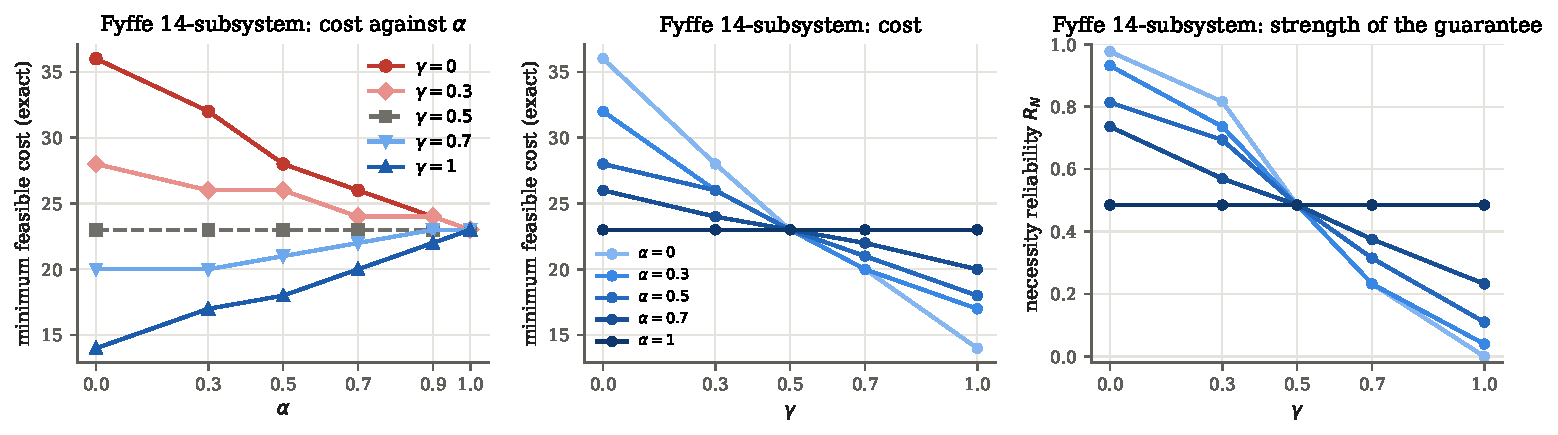
\includegraphics[width=\textwidth]{figS_fyffe_sensitivity.pdf}
\caption{Fyffe-derived instance. Left: minimum feasible cost against $\alpha$, one line per $\gamma$. Center and right: minimum feasible cost and necessity reliability $R_N$ of the prescribed design against $\gamma$, one line per $\alpha$ ($\alpha=0.9$ omitted for legibility). Every point is the certified optimum of its cell.}
\label{fig:supp_fyffe_sensitivity}
\end{figure}

\textbf{Cost and configuration over the grid.} Figure~\ref{fig:supp_fyffe_maps} maps the certified minimum cost and the number of installed subsystems over the $30$ cells. The installed count ranges from $13$ at $(0,0)$ to $7$ at $(0,1)$: the declared attitude changes both the cost of the design and the redundancy it carries.

\begin{figure}[htbp]
\centering
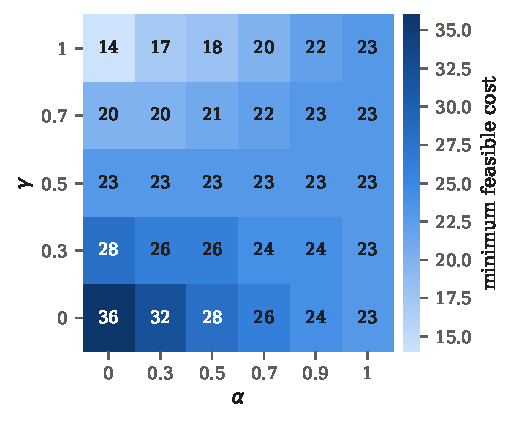
\includegraphics[width=0.48\textwidth]{fig3_cost_heatmap.pdf}\hfill
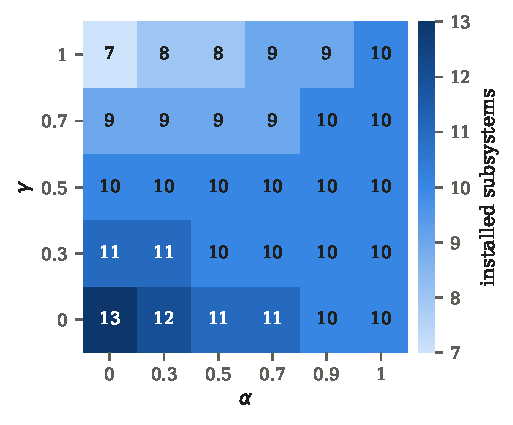
\includegraphics[width=0.48\textwidth]{fig4_config_map.pdf}
\caption{Fyffe-derived instance. Left: certified minimum cost $Z^*(\alpha,\gamma)$. Right: number of subsystems installed by the certified optimum of each cell.}
\label{fig:supp_fyffe_maps}
\end{figure}

\section{Further Results on the IEEE RTS-79 Case Study} \label{sec:supp_rts}

\subsection{The classical readings on the fleet} \label{sec:supp_rts_nesting}
Table~\ref*{M-tab:nesting} of the main article places the classical readings of the success condition at cells of the policy square. Table~\ref{tab:supp_nesting_rts} applies it to the fleet: each reading gives a cell, the cell gives the effective threshold $T$, and the threshold gives the optimal design of the complete parametric solution, so no optimization is solved. The crisp model buys D5 for \$180\,M. Requiring necessity $0.7$ or $0.9$ moves the threshold to $208$ or $216$~MW and buys D7 for \$203\,M, the same fleet as the interval worst case; credibility $0.8$ stops at D6, and the possibility and low-credibility requirements are met by D4 for \$158\,M.

\begin{table}[htbp]
\centering
\caption{The readings of Table~\ref*{M-tab:nesting} of the main article on the IEEE RTS-79 fleet ($\tilde{k} = (162, 180, 198)$~MW, capacity spread $\delta = 0.10$). Each reading is mapped to its cell; $\kappa$ and $T = \lceil\kappa\rceil$ are the effective continuous and integer thresholds in MW, and the design is read from the complete parametric solution (designs D1--D7 of Table~\ref*{M-tab:policy_menu} of the main article). No optimization is solved for this table.}
\label{tab:supp_nesting_rts}
\small
\begin{tabular}{llcrrlrr}
\hline
Reading & Condition & Cell & $\kappa$ & $T$ & Design & Cost (M\$) & $R_N$\\
\hline
Crisp model (modal values) & $W_S \ge k_2$ & $\alpha=1$ & 180.00 & 180 & D5 & 180 & 0.506\\
Interval worst case & $W_{S,L}^{0} \ge k_U^{0}$ & $(0,\,0)$ & 220.00 & 220 & D7 & 203 & 0.951\\
Interval best case & $W_{S,U}^{0} \ge k_L^{0}$ & $(0,\,1)$ & 147.27 & 148 & D1 & 130 & 0.000\\
Necessity & $N(\WS\ge\tilde{k}) \ge 0.7$ & $(0.3,\,0)$ & 207.10 & 208 & D7 & 203 & 0.951\\
Necessity & $N(\WS\ge\tilde{k}) \ge 0.9$ & $(0.1,\,0)$ & 215.60 & 216 & D7 & 203 & 0.951\\
Possibility & $\Pi(\WS\ge\tilde{k}) \ge 0.7$ & $(0.7,\,1)$ & 169.51 & 170 & D4 & 158 & 0.000\\
Credibility & $\mathrm{Cr}(\WS\ge\tilde{k}) \ge 0.3$ & $(0.6,\,1)$ & 166.15 & 167 & D4 & 158 & 0.000\\
Credibility & $\mathrm{Cr}(\WS\ge\tilde{k}) \ge 0.8$ & $(0.4,\,0)$ & 202.98 & 203 & D6 & 180 & 0.617\\
\hline
\end{tabular}
\end{table}


\subsection{Minimum cost against the cut level}
Figure~\ref{fig:sensitivity} plots the certified minimum cost of the RTS-79 fleet over the $30$-cell grid against $\alpha$, one line per $\gamma$; the values are those of Table~\ref*{M-tab:power_rts_stats} of the main article, and the pattern is discussed in its Section~\ref*{M-sec:posture}.

\begin{figure}[!htbp]
\centering
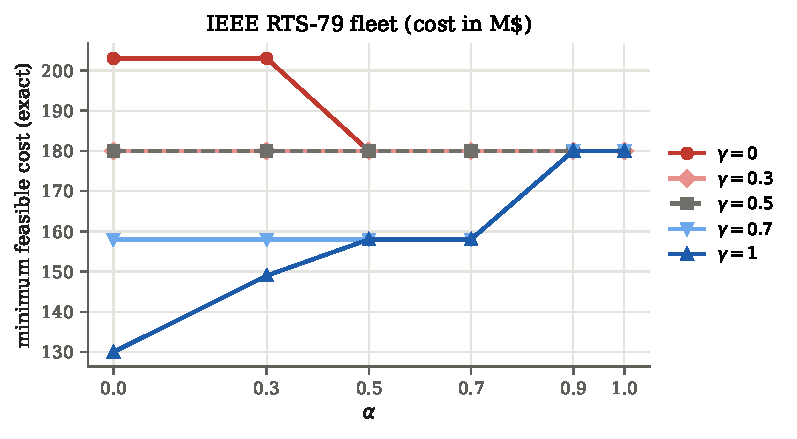
\includegraphics[width=0.75\textwidth]{fig2_cost_sensitivity.pdf}
\caption{\new{Minimum feasible cost against $\alpha$, one line per $\gamma$, for the IEEE RTS-79 fleet. Every point is the certified optimum of its cell; lines overlap where costs coincide. The Fyffe counterpart is Figure~\ref{fig:supp_fyffe_sensitivity}.}}
\label{fig:sensitivity}
\end{figure}

\subsection{Catalog of the fleet} \label{sec:supp_rts_catalog}
Table~\ref{tab:rts_catalog} lists the complete discrete catalog of the case study of Section~\ref*{M-sec:rts_benchmark} of the
main article. Option~0 is the null option; hydro units are available only at Bays~3--6.

\begin{table}[!htbp]
\centering
\caption{Complete 10-bay discrete option catalog for the IEEE RTS-79 generation fleet case study. Option~0 represents an uncommitted (null) bay $(w=0, c=0, p=0)$. Unit classes and availability parameters $p_{i,j} = 1 - \text{FOR}_i$ are from RTS-79; capital costs are illustrative engineering estimates.}
\label{tab:rts_catalog}
\footnotesize
\setlength{\tabcolsep}{5pt}
\begin{tabular}{cclccc}
\hline
\textbf{Bay} $i$ & \textbf{Option} $j$ & \textbf{Generating Unit Class} & \textbf{Capacity} $w_{i,j}$ (MW) & \textbf{Capital Cost} $c_{i,j}$ (\$M) & \textbf{Availability} $p_{i,j}$\\
\hline
1--2 & 1 & 12~MW Oil Steam & 12 & 14 & 0.980\\
     & 2 & 20~MW Combustion Turbine & 20 & 18 & 0.900\\
\hline
3--4 & 1 & 20~MW Combustion Turbine & 20 & 18 & 0.900\\
     & 2 & 50~MW Hydro & 50 & 45 & 0.990\\
\hline
5--6 & 1 & 50~MW Hydro & 50 & 45 & 0.990\\
     & 2 & 76~MW Coal Steam & 76 & 68 & 0.980\\
\hline
7--8 & 1 & 76~MW Coal Steam & 76 & 68 & 0.980\\
     & 2 & 100~MW Oil Steam & 100 & 85 & 0.960\\
\hline
9--10 & 1 & 100~MW Oil Steam & 100 & 85 & 0.960\\
      & 2 & 155~MW Coal Steam & 155 & 135 & 0.960\\
\hline
\end{tabular}
\end{table}


\subsection{Reliability target} \label{sec:supp_rts_rtarget}
At $\Rtarget = 0.95$ the cost-minimizing fleets of the
optimistic boundary, modal and necessity cells are series arrangements at their threshold $T$: the loss of any single unit drops the
working capacity below $T$. Table~\ref{tab:rts_rtarget_sensitivity} repeats the optimization for
$\Rtarget \in \{0.90, 0.91, \dots, 0.99\}$ at the thresholds of the optimistic boundary cell $(0,1)$
($T=148$~MW), the modal cell $(0.5,0.5)$ ($T=180$~MW) and the necessity cell $(0,0)$ ($T=220$~MW).

\begin{table}[!htbp]
\centering
\caption{Sensitivity of the optimal fleet to the reliability target $R_{\mathrm{target}} \in \{0.90, 0.91, \dots, 0.99\}$ on the IEEE RTS-79 fleet at three effective thresholds. Consecutive targets with the same optimal design are merged. $R_{\mathrm{sys}}$ is the reliability at the effective threshold $T$. The last column states whether the working capacity still reaches $T$ after the loss of the largest installed unit, and gives that remaining capacity.}
\label{tab:rts_rtarget_sensitivity}
\scriptsize
\setlength{\tabcolsep}{1.5pt}
\begin{tabular}{lcp{4.4cm}cccc}
\hline
Regime & $R_{\mathrm{target}}$ & Optimal fleet & MW & Cost (M\$) & $R_{\mathrm{sys}}$ & Largest-unit loss\\
\hline
\multirow{3}{*}{\shortstack[l]{Optimistic boundary\\$(0,1)$, $T=148$~MW}} & 0.90--0.95 & 1 $\times$ 50 MW Hydro + 1 $\times$ 100 MW Oil & 150 & 130 & 0.9504 & No (50 MW)\\
 & 0.96--0.97 & 3 $\times$ 50 MW Hydro & 150 & 135 & 0.9703 & No (100 MW)\\
 & 0.98--0.99 & 4 $\times$ 50 MW Hydro & 200 & 180 & 0.9994 & Yes (150 MW)\\
\hline
\multirow{4}{*}{\shortstack[l]{Modal\\$(0.5,0.5)$, $T=180$~MW}} & 0.90--0.92 & 1 $\times$ 76 MW Coal + 1 $\times$ 100 MW Oil + 1 $\times$ 12 MW Oil & 188 & 167 & 0.9220 & No (88 MW)\\
 & 0.93--0.94 & 2 $\times$ 50 MW Hydro + 1 $\times$ 76 MW Coal + 1 $\times$ 12 MW Oil & 188 & 172 & 0.9413 & No (112 MW)\\
 & 0.95--0.96 & 4 $\times$ 50 MW Hydro & 200 & 180 & 0.9606 & No (150 MW)\\
 & 0.97--0.99 & 4 $\times$ 50 MW Hydro + 1 $\times$ 12 MW Oil + 1 $\times$ 20 MW CT & 232 & 212 & 0.9948 & Yes (182 MW)\\
\hline
\multirow{4}{*}{\shortstack[l]{Necessity\\$(0,0)$, $T=220$~MW}} & 0.90--0.93 & 1 $\times$ 50 MW Hydro + 1 $\times$ 76 MW Coal + 1 $\times$ 100 MW Oil & 226 & 198 & 0.9314 & No (126 MW)\\
 & 0.94--0.95 & 3 $\times$ 50 MW Hydro + 1 $\times$ 76 MW Coal & 226 & 203 & 0.9509 & No (150 MW)\\
 & 0.96--0.97 & 4 $\times$ 50 MW Hydro + 1 $\times$ 76 MW Coal & 276 & 248 & 0.9794 & No (200 MW)\\
 & 0.98--0.99 & 4 $\times$ 50 MW Hydro + 1 $\times$ 76 MW Coal + 1 $\times$ 20 MW CT & 296 & 266 & 0.9967 & Yes (220 MW)\\
\hline
\end{tabular}
\end{table}


A fleet that still reaches $T$ after the loss of its largest unit becomes optimal at $\Rtarget = 0.97$
in the modal cell (\$212\,M, $232$~MW, $\Rsys = 0.9948$) and at $\Rtarget = 0.98$ in the other two
cells (\$180\,M and $200$~MW in the optimistic boundary cell; \$266\,M and $296$~MW in the necessity cell).
For lower targets no optimal fleet tolerates the loss of its largest unit. In the modal cell three designs are
optimal below that point: \$167\,M up to $\Rtarget = 0.92$, \$172\,M at
$0.93$--$0.94$ and \$180\,M at $0.95$--$0.96$. These breakpoints are properties of this catalog and target
range, not general rules.


\subsection{Unit-specific capacity spreads} \label{sec:supp_rts_unit}
This section gives the full results summarized in Section~\ref*{M-sec:robustness} of the main article.


The baseline RTS-79 formulation of Section~\ref*{M-sec:rts_benchmark} of the main article gives every candidate unit the same proportional spread $\delta = 0.10$, which is the hypothesis under which Theorem~\ref*{M-thm:reduction} holds. The sources of capacity imprecision do not, however, affect all generating technologies alike, and for one of them RTS-79 is explicit. Its Table~6 gives the available capacity of the hydro units as $100\%$ of the $50$~MW rating in the first two quarters of the year and $90\%$ in the last two, so the hydro capacity is the triangular number $(45, 50, 50)$~MW, that is $(\delta_l,\delta_r) = (0.10, 0)$: the same downside as the common spread and no upside. For thermal units RTS-79 reports full outages only and leaves partial outages to the user (note to its Table~4), so we assume spreads that encode the qualitative effect of ambient temperature: $(0.15, 0.05)$ for the 20~MW combustion turbines, whose output falls as combustion air density drops, and $(0.05, 0.02)$ for the oil- and coal-fired steam units (12, 76, 100 and 155~MW), which are limited by condenser back-pressure. The thermal values are an assumption of this study, chosen to reflect the qualitative ordering rather than measured derating curves; how much the results depend on them is reported below.

With heterogeneous spreads the hypothesis of Theorem~\ref*{M-thm:reduction} fails. The effective threshold is no longer a single closed-form function of $(\alpha,\gamma)$, so each policy cell must be solved by the unreduced exact search on the component-specific $\alpha$-cut intervals $[w_{i,L}^\alpha, w_{i,U}^\alpha]$. With a time limit of $600$~s per cell, all $30$ cells complete; the slowest takes $234$~s, whereas every cell of the reduced formulation solves in at most $0.01$~s of solver time (Section~\ref*{M-sec:scaling} of the main article). As a check on the implementation, the unreduced search with every unit spread set to $0.10$ reproduces the reduced optimum in each of the three cells tested, and an independent exhaustive enumeration of all $3^{10}$ fleets in exact rational arithmetic reproduces four of the optima reported below and the \$171\,M fleet discussed at the end of this section (Section~\ref{sec:supp_pipeline}). Table~\ref{tab:rts_unit_specific} lists every cell in which the optimum changes. It also decomposes each change: in the ``thermal only'' column the thermal units receive their unit-specific spreads while hydro keeps the common spread, and in the ``hydro only'' column the reverse.

\begin{table}[!htbp]
\providecommand{\revtablecolor}{}\revtablecolor
\centering
\caption{Policy cells of the IEEE RTS-79 fleet in which unit-specific capacity spreads change the optimal fleet relative to the common spread $\delta=0.10$. Unit-specific spreads: hydro $(\delta_l,\delta_r)=(0.10,0)$ from RTS-79 Table~6; combustion turbine $(0.15,0.05)$ and steam units $(0.05,0.02)$, an assumption of this study. ``Thermal only'' changes the thermal units and keeps hydro at the common spread; ``hydro only'' does the reverse.}
\label{tab:rts_unit_specific}
\footnotesize
\begin{tabular}{ccp{3.0cm}p{3.0cm}cccc}
\hline
$\alpha$ & $\gamma$ & Common-spread fleet & Unit-specific fleet & Common & Thermal only & Hydro only & Unit-specific\\
\hline
0.3 & 0.0 & 3 $\times$ 50 MW hydro + 1 $\times$ 76 MW coal & 1 $\times$ 50 MW hydro + 1 $\times$ 155 MW coal & \$203\,M & \$180\,M & \$203\,M & \$180\,M\\
0.0 & 0.3 & 4 $\times$ 50 MW hydro & 1 $\times$ 50 MW hydro + 1 $\times$ 155 MW coal & \$180\,M & \$180\,M & \$180\,M & \$180\,M\\
0.3 & 0.7 & 2 $\times$ 50 MW hydro + 1 $\times$ 76 MW coal & 4 $\times$ 50 MW hydro & \$158\,M & \$158\,M & \$158\,M & \$180\,M\\
0.5 & 0.7 & 2 $\times$ 50 MW hydro + 1 $\times$ 76 MW coal & 4 $\times$ 50 MW hydro & \$158\,M & \$158\,M & \$171\,M & \$180\,M\\
0.7 & 0.7 & 2 $\times$ 50 MW hydro + 1 $\times$ 76 MW coal & 4 $\times$ 50 MW hydro & \$158\,M & \$180\,M & \$180\,M & \$180\,M\\
0.0 & 1.0 & 1 $\times$ 50 MW hydro + 1 $\times$ 100 MW oil & 3 $\times$ 50 MW hydro + 1 $\times$ 12 MW oil & \$130\,M & \$135\,M & \$135\,M & \$149\,M\\
0.3 & 1.0 & 3 $\times$ 50 MW hydro + 1 $\times$ 12 MW oil & 2 $\times$ 50 MW hydro + 1 $\times$ 76 MW coal & \$149\,M & \$149\,M & \$158\,M & \$158\,M\\
\hline
\multicolumn{8}{p{\dimexpr\linewidth-2\tabcolsep\relax}}{\textit{Note}: 7 of 30 cells differ; 0 timed out at 600\,s. In 7 of the 7 differing cells the unit-specific optimum coincides with the crisp optimum of some integer threshold (library: 73 thresholds, 7 distinct designs). Unreduced solve time per cell: $0.008$--$234$\,s; reduced formulation: $\le 0.01$\,s per cell.}\\
\hline
\end{tabular}
\end{table}


The optimal fleet changes in $7$ of the $30$ cells and its cost in $6$, in both directions.
\begin{itemize}
\item \emph{Necessity side: over-investment.} At $(0.3, 0.0)$ the common spread prescribes three hydro units and one 76~MW coal unit at \$203\,M, and the unit-specific model one hydro unit and one 155~MW coal unit at \$180\,M, a saving of \$23\,M ($11.3\%$). The saving is due to the thermal spreads alone; the hydro values of Table~6 change nothing there. In the necessity cell $(0.0, 0.0)$ the optimum is unchanged, because on the downside a hydro unit is worth $45$~MW under Table~6 exactly as under the common spread. At $(0.0, 0.3)$ the fleet changes at equal cost.
\item \emph{Possibility side: under-investment.} In five cells the common spread lets upper-bound capacities satisfy the requirement too cheaply, and the unit-specific model requires more capital: $+\$19$\,M at $(0.0, 1.0)$, $+\$9$\,M at $(0.3, 1.0)$, and $+\$22$\,M at $(0.3, 0.7)$, $(0.5, 0.7)$ and $(0.7, 0.7)$. The main driver is the missing hydro upside: the common spread credits a hydro unit with up to $55$~MW, Table~6 with at most $50$. The decomposition shows that the two sources interact. At $(0.3, 1.0)$ the hydro change alone accounts for the difference and at $(0.7, 0.7)$ either change alone suffices, but at $(0.0, 1.0)$ each change on its own raises the cost only to \$135\,M, and at $(0.3, 0.7)$ neither change on its own moves the optimum; the full increase arises only when both are applied.
\end{itemize}
In the remaining $23$ cells the prescribed fleet is unchanged.

\textbf{Matched common-spread controls.} To check whether the seven changed optima arise from unit-level heterogeneity or from a smaller aggregate spread, we evaluated all 30 cells against a single common-spread control $(\delta_l, \delta_r) = (0.06, 0.02)$ applied to every unit.
Under the matched control, exactly 5 of the 7 discrepancies with the baseline common spread are reproduced identically. The two remaining cells are $(0.0, 0.3)$ and $(0.3, 0.7)$. In $(0.0, 0.3)$ the cost is unchanged (\$180\,M) but the fleet is not: the unit-specific hydro spread has no upside, so at the effective demand $k^0(0.3) = 187.2$~MW four hydro units supply only $4 \times (0.3 \cdot 50 + 0.7 \cdot 45) = 186$~MW, and the equal-cost D6 replaces D5. Cell $(0.3, 0.7)$ is the least robust cell of the table (see below). With this one control, most of the changes are reproduced by a smaller common spread; separating magnitude from heterogeneity in general would require a sweep over common spreads.

\textbf{Sensitivity to the spread values.} Varying the hydro downside ($\delta_l \in \{0, 0.02, 0.05, 0.10\}$, with $\delta_r = 0$) leaves the optimum unchanged in six of the seven cells; at $(0.3, 0.7)$ the cost is \$158\,M for $\delta_l \le 0.02$ and \$180\,M from $0.05$. Varying the assumed thermal spreads (the combustion-turbine downside over $\{0.10, 0.15, 0.20\}$ or the steam downside over $\{0.02, 0.05, 0.08\}$) leaves the optimum unchanged in six cells, including the necessity-side saving at $(0.3, 0.0)$. The exception is again $(0.3, 0.7)$: with a combustion-turbine downside of $0.10$, or a steam downside of $0.02$, the optimum becomes a \$171\,M fleet of one 155~MW coal unit and two 20~MW combustion turbines. Cell $(0.3, 0.7)$ is therefore the least robust result of the table, and the necessity-side saving the most robust.

\textbf{Relation to Theorem~\ref*{M-thm:reduction}.} At the spreads of Table~\ref{tab:rts_unit_specific}, every one of the seven unit-specific optima coincides with the crisp optimum of some integer threshold: it belongs to the library of optima of the $73$ integer thresholds of Section~\ref*{M-sec:parametric} of the main article, which contains only $7$ distinct designs. That coincidence is not general. The \$171\,M fleet that appears at $(0.3, 0.7)$ under the perturbed thermal spreads, and at $(0.5, 0.7)$ in the hydro-only variant, is the crisp optimum of no integer threshold; the exhaustive enumeration confirms both its optimality and its absence from the library. Heterogeneous spreads can therefore select a design that no single effective threshold would. The common-spread model then cannot represent the optimal design, which only the unreduced search finds.




\section{Model Baselines: Details} \label{sec:supp_baselines}
Section~\ref*{M-sec:baselines_def} of the main article defines the model baselines and Section~\ref*{M-sec:baselines_res} reports their main results.
Table~\ref{tab:supp_baselines} gives the decision-level baselines in full, including the share of the
square on which the baseline design is also optimal and the area-weighted mean cost excess, and
Table~\ref{tab:supp_probabilistic} the probabilistic counterpart under both densities.

On the RTS-79 fleet the three decision-level baselines fail on the same region, on which the dual
threshold exceeds $200$~MW and every baseline prescribes the four-hydro design D5. Elsewhere the crisp
design is D5 at every posture and is optimal on the $61.1\%$ of the square on which D5 is optimal; the
one-sided models track part of the variation of the threshold and are optimal on about three quarters
of the square. On the derived instances, whose libraries contain $29$ and $20$ designs, the one-sided
models fail on a third of the square and the crisp design on half.

The probabilistic designs meet the target under the declared rule only up to an effective threshold of
$200$~MW on the RTS-79 fleet and $41$ on the Pharmaceutical-derived instance; the random threshold
exceeds these values with probability $0.034$ and $0.373$ under triangular densities. Each probabilistic
design is optimal at no posture of the square. The choice of density changes the design on both
instances, while its threshold coverage and its failure and higher-cost shares over the square stay the same; the largest cost excess changes slightly.

\begin{table}[!htbp]
\centering
\caption{Decision-level model baselines in full (shares of the part of the policy square on which some design meets the target). ``Optimal'': the baseline design is also optimal under the declared rule; ``Mean excess'': area-weighted relative cost excess over the part on which the baseline design meets the target, including the part on which it is optimal.}
\label{tab:supp_baselines}
\footnotesize
\setlength{\tabcolsep}{4pt}
\begin{tabular}{llrrrrr}
\hline
Instance & Baseline & Fails & Costlier & Optimal & Max.\ excess & Mean excess\\
 & & (\%) & (\%) & (\%) & (\%) & (\%)\\
\hline
RTS-79 & Crisp & 6.8 & 32.1 & 61.1 & 38.5 & 5.5\\
 & Fuzzy capacities only & 6.8 & 17.1 & 76.1 & 21.5 & 2.2\\
 & Fuzzy demand only & 6.8 & 16.7 & 76.5 & 21.5 & 2.1\\
\hline
Fyffe-derived & Crisp & 50.0 & 37.6 & 12.4 & 64.3 & 12.0\\
 & Fuzzy capacities only & 37.7 & 37.6 & 24.7 & 42.9 & 6.6\\
 & Fuzzy demand only & 33.0 & 27.7 & 39.3 & 21.4 & 2.8\\
\hline
Pharma-derived & Crisp & 49.9 & 33.4 & 16.7 & 33.7 & 5.5\\
 & Fuzzy capacities only & 33.5 & 33.4 & 33.1 & 25.0 & 3.0\\
 & Fuzzy demand only & 30.9 & 30.3 & 38.8 & 16.3 & 1.9\\
\hline
\end{tabular}
\end{table}

\begin{table}[!htbp]
\centering
\caption{Probabilistic counterpart: optimal design under triangular and uniform densities on the supports of the fuzzy data, the largest effective threshold at which it meets the target, the probability that the random threshold exceeds it, and its evaluation over the policy square under the declared rule. Pharmaceutical designs are given as option vectors.}
\label{tab:supp_probabilistic}
\footnotesize
\setlength{\tabcolsep}{2.5pt}
\begin{tabular}{llp{3.3cm}rrrrrrr}
\hline
Instance & Density & Design & Cost & $R_{\mathrm{prob}}$ & $T$ met & $\Pr\{\hat{T}>\cdot\}$ & Fails & Costlier & Max.\ exc.\\
 & & & & & & & (\%) & (\%) & (\%)\\
\hline
RTS-79 & triangular & 4$\times$50~MW hydro + 1$\times$12~MW oil & 194 & 0.9605 & 200 & 0.034 & 6.8 & 93.2 & 49.2\\
 & uniform & 4$\times$50~MW hydro + 1$\times$20~MW CT & 198 & 0.9587 & 200 & 0.112 & 6.8 & 93.2 & 52.3\\
Pharma-derived & triangular & (0, 2, 1, 1, 1, 2, 0, 2, 1, 2) & 133 & 0.8513 & 41 & 0.373 & 33.5 & 66.5 & 44.6\\
 & uniform & (0, 2, 1, 1, 2, 2, 0, 2, 1, 2) & 135 & 0.8541 & 41 & 0.417 & 33.5 & 66.5 & 46.7\\
\hline
\end{tabular}
\end{table}


\bibliographystyle{elsarticle-harv}
\bibliography{sn-bibliography}

\end{document}
